\documentclass[11pt]{homework}
\usepackage[utf8]{inputenc}
\usepackage{graphicx}
\usepackage{wrapfig}
\usepackage[table]{xcolor}
\usepackage{biblatex}
\usepackage{abstract}
\addbibresource{bibliography.bib}
\renewcommand{\linespread}{1.0}

\begin{document}

\title{COMP-551 Mini-Project 3 \and COMP-551 Winter 2021}
\author{Arneet Singh Kalra, Behnaz Ghefati Feizabadi, Hussein Lakkis}
\date{April 1, 2021}
\maketitle{}

\begin{abstract}
\normalsize
Neural networks are powerful tools to model complex patterns in large databases. In this project, we implemented a neural network, the Multilayer Perceptron, to classify image data from the MNIST (Modified National Institute of Standards and Technology) Dataset containing handwritten digits. A variety of experiments tested the performance of the network with varying hidden layers and respective units, activation functions and the use of regularization. Our results showed that the model performed best with 2 hidden layers of 256 units using ReLU activations, achieving a testing accuracy of 98.19\%. Increasing the number of hidden layers with ReLU activations up to 2 layers resulted in an overall increase in testing accuracy. Furthermore, increasing the width of the hidden layers also increased testing accuracy for MLPs with both ReLU and Tanh activations, but not for Sigmoid functions which capped at 128 units. Lastly, using L2 regularization on the MNIST dataset decreased testing accuracy, likely a result of overregularization. 
\end{abstract}

\section{Introduction}

\subsection{Project Background and Goals}
The goal of this project is to implement a Multilayer Perceptron, and train and test it on the MNIST Dataset of handwritten digits. The original dataset comes from the National Institute of Standards and Technology, a branch of the United States Department of Commerce. The dataset was normalized to fit into a 28 by 28 pixel bounding box and anti-aliased, resulting in a gray-scale. This modified dataset is commonly used in training machine learning algorithms. In our experiments, we tested a variety of different activations functions, learning rates, number of hidden layers, varying layer widths, and other key metrics such as L2 regularization. Our best model resulted in an accuracy of 98.19\%. The model used a learning rate of 0.01, 2 hidden layers, 512 units in each layer, and ReLU activations. The model performed the worst on unnormalized images, with a testing accuracy of 11.46\% (slightly better than random chance). Using a ReLU activation, increasing the number of hidden layers up to 2 and the number of units in each hidden layer, increased the testing accuracy. However, adding L2 regularization to the cost decreased the accuracy of the network. 

\subsection{Discussion of Related Work}
The MNIST dataset is a popular set used in academics to test different models. In this project, we developed a Multilayer Perceptron, however there exist a variety of neural networks which can be trained on this dataset. At the time of this project, one of the most efficient set of models are Convolutional Neural Networks (CNNs). A study by Kumar et al. showcases their CNN model which is composed of multiple convolutions and pooling layers alongisde ReLU activations \cite{garg2019validation}. The CNN models performs exceptionally well, receiving a test accuracy greater than 98\% \cite{garg2019validation}. In the original paper where MNIST dataset was used, a Support Vector Machine was able to achieve an error rate of 0.8\% \cite{lecun1998gradient}.While examining other articles, we came across a variety of other real-life applications for MLPs. A study published in the Journal of Food Engineering uses MLPs to model the soaking characteristics of wheat kernel at varying temperatures. The soaking temperature and time were used as input parameters and the moisture ratio was used as output parameter \cite{kashaninejad2009modeling}. The resulting network performed relatively well when compared to the actual experimental data. Another paper from Boughara et al. describes the use of an a single hidden layer MLP in facial recognition applications to classify facial expressions from three large datasets \cite{boughrara2016facial}. The results of the study clearly demonstrate the efficiency of their model. 


\section{Dataset}
The MNIST dataset contains 60 000 training images and 10 000 testing images of handwritten digits between 0 and 9. Each image is a 28 x 28 pixel bounded box, encompassed as a 2D array. Each value in the array represents the gray-scale factor of the pixel, a value between 0 and 255, as visualized in Figure \ref{digit-png}.  Figure \ref{pxiel-dist} shows the distribution of the values between 0 and 255. As expected, a majority of the pixels contain a value of 0, representing no part of the digit present at the respective pixel. Therefore, during the pre-processing of the data, the digits were first normalized to have values between 0.0 and 1.0. This step of normalization reduces the complexity of the model, improves the accuracy, speeds up the training time, and reduces variance. Then, the images were flattened to convert the 2D array into a one dimensional array, the input vector, of size 784. Finally, for a majority of the experiments, 10 000 data samples from the training set were isolated as the validation set, leaving 50 000 for training.

\begin{figure}[h!]
  \centering
  \begin{minipage}[h]{0.3\textwidth}
    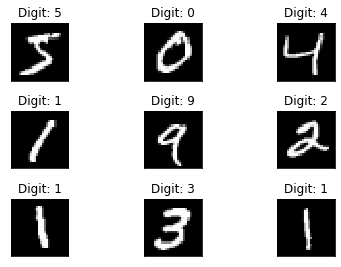
\includegraphics[width=\textwidth]{example-digits.png}
     \caption{Sample Handwritten Digits}
     \label{digits-png}
  \end{minipage}
\hfill
  \begin{minipage}[h]{0.3\textwidth}
    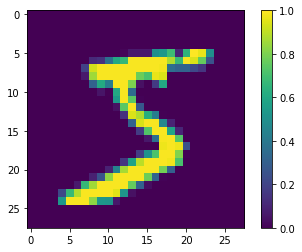
\includegraphics[width=\textwidth]{example-digit.png}
     \caption{Handwritten Digit from Dataset Colourized}
     \label{digit-png}
  \end{minipage}
\hfill
    \begin{minipage}[h]{0.3\textwidth}
    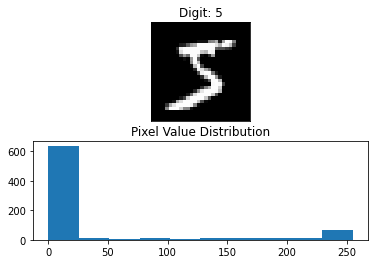
\includegraphics[width=\textwidth]{pixel-distribution.png}
    \caption{Pixel Distribution of a Digit in MNIST}
    \label{pxiel-dist}
  \end{minipage}
\end{figure}

\section{Results}
\subsection{Varying Number of Hidden Layers with ReLU Activation}
In our first experiment, we ran three iterations of our model: 0 hidden layers, 1 hidden layer, and 2 hidden layers. The MLPs with hidden layers used ReLU activations, and since we are performing classification, had a Softmax layer at the end. Each hidden layer had 128 units. By monitoring the training accuracy against the number of iterations, we concluded that the training accuracy started to stay constant after 60 epochs for 0 and 1 hidden layers. An epoch of 40 was used for 2 hidden layers. Then, hyperparameter tuning was performed on each model to find the optimal learning rate, as demonstrated by figures \ref{hyper-0} to \ref{hyper-2-128-relu}. All 3 models performed best using a learning rate of 0.1. As indicated by Table \ref{table-varying-hidden-layers}, the best model out of the three used 2 hidden layers and received a test accuracy of 98.01\%. It also received a perfect training accuracy. On the other hand, the model with no hidden layers performed the worst among the three, receiving a testing and training accuracy lower than or equal to 93\%. Therefore, we see that with more hidden layers, our results are more accurate. The reason for this is perhaps using softmax regression (no hidden layers) does not capture the complexity of the data. Therefore, when hidden layers are added, and non-linearities are applied, the complex feature (vertical edges, or patterns) are resolved, thus getting a better-fit model. It is worth mentioning that adding additional hidden layers might lead to an overfit model.

\begin{table}[h!] 
\centering
\begin{tabular}{||c c c||} 
\hline
 # Hidden Layers & Train Accuracy & Test Accuracy(\%) \\ [0.5ex]
 \hline\hline
 0  & 93.00  & 92.54   \\ 
 1  & 99.93  & 97.79   \\ 
 2  & 100.00 & 98.01   \\ 
 \hline
\end{tabular}
\caption{Varying Number of Hidden Layers Effect on Test Accuracy}
\label{table-varying-hidden-layers}
\end{table}

\begin{figure}[h!]
  \centering
  \begin{minipage}[h]{0.3\textwidth}
    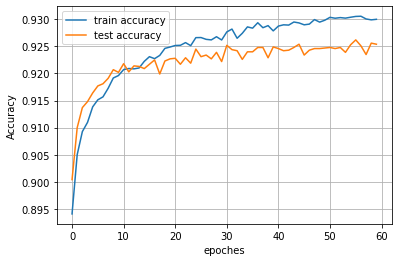
\includegraphics[width=\textwidth]{acc-0.png}
    \caption{No Hidden Layer Accuracies}
    \label{acc-0}
  \end{minipage}
\hfill
   \begin{minipage}[h]{0.3\textwidth}
    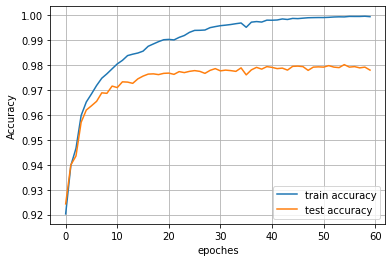
\includegraphics[width=\textwidth]{acc-1-128-relu.png}
    \caption{128 unit Hidden Layer ReLU Accuracies}
    \label{acc-1-128-relu}
  \end{minipage}
\hfill
   \begin{minipage}[h]{0.3\textwidth}
    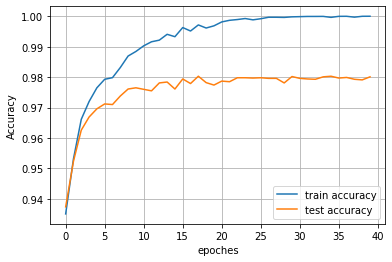
\includegraphics[width=\textwidth]{acc-2-128-relu.png}
    \caption{128 unit 2 Hidden Layers ReLU Accuracies}
    \label{acc-2-128-relu}
  \end{minipage}
\end{figure}

\begin{figure}[h!]
  \centering
  \begin{minipage}[h]{0.3\textwidth}
    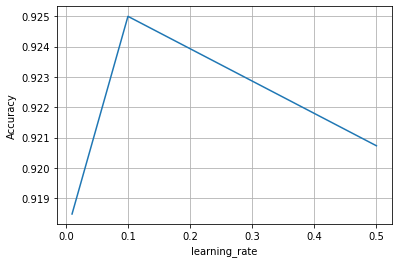
\includegraphics[width=\textwidth]{hyper-0.png}
    \caption{No Hidden Layer Tuning}
    \label{hyper-0}
  \end{minipage}
\hfill
   \begin{minipage}[h]{0.3\textwidth}
    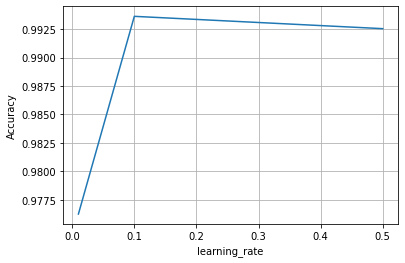
\includegraphics[width=\textwidth]{hyper-1-128-relu.png}
    \caption{128 unit Hidden Layer ReLU Tuning}
    \label{hyper-1-128-relu}
  \end{minipage}
\hfill
   \begin{minipage}[h]{0.3\textwidth}
    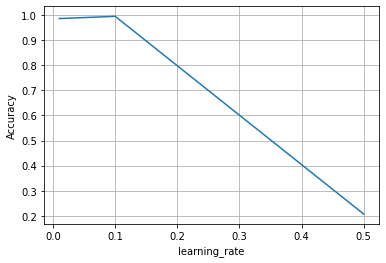
\includegraphics[width=\textwidth]{hyper-2-128-relu.png}
    \caption{128 unit 2 Hidden Layers ReLU Tuning}
    \label{hyper-2-128-relu}
  \end{minipage}
\end{figure}





\subsection{Varying Activation Functions}
Using the same model as above with 2 hidden layers and 128 units, we ran experiments with 2 other types of activation functions: Sigmoid and Hyperbolic tangent. Hyperparameter tuning was performed on the two models to find the optimal learning rate. The Sigmoid activation function model performed best with a 0.5 learning rate, whereas the Tanh model was best with 0.1 just as the ReLU model. Figure \ref{exp-2-sigmoid} and \ref{exp-2-tanh} plot the accuracy of the Sigmoid and Hyperbolic tangent MLPs respectively, relative to epochs. Our results showed that the Sigmoid model performed the best, achieving a test accuracy of 98.09\%. The ReLU model performed a tad lower with a test accuracy of 98.01\%. However, all results are approximately the same and therefore no difference was observed. This might be due to random chance.

\begin{table}[h!] 
\centering
\begin{tabular}{||c c c c||} 
\hline
 # Activation Function & Learning Rate & Train Accuracy & Test Accuracy(\%) \\ [0.5ex]
 \hline\hline
 ReLU     & 0.1 & 100.00 & 98.01   \\
 Sigmoid  & 0.5 & 99.98  & 98.09   \\ 
 Tanh     & 0.1 & 100.00 & 98.04   \\ 
 \hline
\end{tabular}
\caption{Varying Activation Function Effect on Test Accuracy}
\label{table-varying-activations}
\end{table}

\begin{figure}[h!]
  \centering
  \begin{minipage}[h]{0.4\textwidth}
    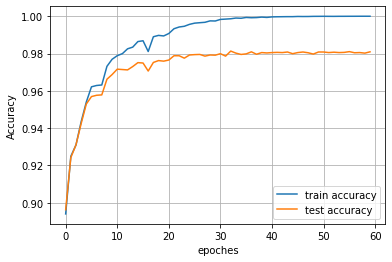
\includegraphics[width=\textwidth]{acc-2-128-sigmoid.png}
     \caption{Accuracy of Sigmoid Activation}
     \label{exp-2-sigmoid}
  \end{minipage}
\hspace{1.5cm}
   \begin{minipage}[h]{0.4\textwidth}
    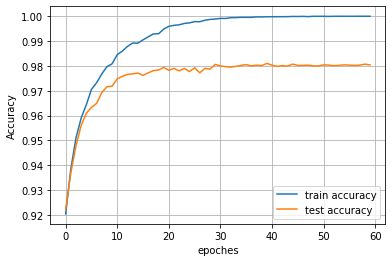
\includegraphics[width=\textwidth]{acc-2-128-tanh.png}
    \caption{Accuracy of Tanh Activation}
    \label{exp-2-tanh}
  \end{minipage}
\end{figure}






\subsection{L2 Regularization}
In this experiment, we added L2 regularization to the cost of the MLP with 2 hidden layers using ReLU activations. During the hyperparameter tuning, we tested learning rates of 0.01 and 0.1, as well as lambda values of 0.3, 0.1 and 0.01. Figure \ref{exp-3-tuning} plots the parameters with their respective accuracies. Our optimal values are 0.1 for the learning rate and 0.01 for lambda. With these parameters, our model received a training accuracy of 97.33\% and a testing accuracy of 97.05\%. Comparing this to the model without L2 regularization, this modification to the cost resulted in a decrease of testing accuracy by 0.96\%. One reason might be that regularization with the hyper-parameters and activation functions we have might be leading to over-fitting. Moreover, neural networks have more than one minimum and with the learning rate and activation functions used, we might be converging to a local optimum. RelU might not be the best function here. More experiments should be done to test the effect of regularization. 

\begin{figure}[h!]
  \centering
  \begin{minipage}[h]{0.4\textwidth}
    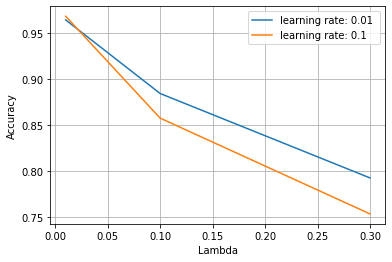
\includegraphics[width=\textwidth]{hyper-l2-reg.png}
     \caption{Hyperparameter Tuning of L2 Regularization Model}
     \label{exp-3-tuning}
  \end{minipage}
\hspace{1.5cm}
  \begin{minipage}[h]{0.4\textwidth}
    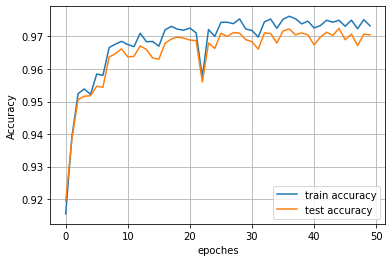
\includegraphics[width=\textwidth]{acc-l2-reg.png}
    \caption{Accuracy with L2 Regularization}
    \label{exp-3-accuracy}
  \end{minipage}
\end{figure}





\subsection{Unnormalized Images}
\begin{wrapfigure}{r}{0.3\textwidth} %this figure will be at the right
    \centering
    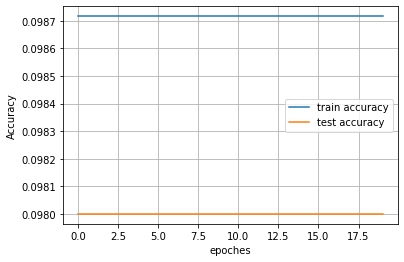
\includegraphics[width=0.3\textwidth]{acc-unnoramlized.png}
    \caption{Accuracy with Unnormalized Data }
    \label{exp-4-acc}
\end{wrapfigure}
This model used 2 hidden layers with 128 units and ReLU activations, but was trained using unnormalized images. Therefore the range of each value in the unit vector is between 0 and 255. Using 20 epoches and a learning rate of 0.1, the model resulted in a training accuracy of 9.87\% and a test accuracy of 9.80\%. This is to be expected since we now have values ranging up to 255 in the input vector. These values result in the weight sum of the layer to be far from 0 taking away the non-linear aspect of the activation function. 



\subsection{Additional Experiments}
\subsubsection{Varying Widths of Hidden Layers}
We investigated the effect that the width of the hidden layers has on the testing accuracy. During the experiments, we tested 64, 128, 256 and 512 unit hidden layers with ReLU activations. For the models with Sigmoid and Tanh activations, we test 2 hidden layers and tested 64, 128, and 526 units.  Table \ref{table-hidden-units} shows the results of our various experiments. We achieve the best test accuracy of 98.19\% using 2 hidden layers with 512 units each and a ReLU activation function. Using 256 units instead on the same model results a 0.02\% lower accuracy. With the models using Tanh, the most accurate result is using a hidden layer width of 256 units. However, for the model with the Sigmoid function, 256 units is the least accurate: the most accurate uses a hidden layer width of 128 units.

\begin{table}[h!] 
\centering
\begin{tabular}{||c c c c||} 
\hline
 # Hidden Layers & Units & Activations &  Test Accuracy(\%) \\ [0.5ex]
 \hline\hline
 0 & -   & -          & 92.54   \\ 
\hline
 1 & 64  & ReLU       & 97.47   \\
 1 & 128 & ReLU       & 97.79   \\
 1 & 256 & ReLU       & 97.99   \\
 1 & 512 & ReLU       & 98.09   \\
 2 & 64  & ReLU       & 97.79   \\
 2 & 128 & ReLU       & 98.01   \\
 2 & 256 & ReLU       & 98.17   \\
 2 & 512 & ReLU       & 98.19   \\ 
\hline
 2 & 64  & Tanh       & 97.64   \\
 2 & 128 & Tanh       & 97.99   \\
 2 & 256 & Tanh       & 98.16   \\
\hline
 2 & 64  & Sigmoid    & 97.27   \\ 
 2 & 128 & Sigmoid    & 98.09   \\ 
 2 & 256 & Sigmoid    & 97.17   \\ 
 \hline
\end{tabular}
\caption{Accuracies of Varying Number of Units in Hidden Layer(s)}
\label{table-hidden-units}
\end{table}

\subsubsection{Varying Number of Training Images}
Lastly, we observed the test accuracy based on the number of training images used. Tested values are 10$^k$ where  k $\in$ {0, 1, 2, 3, 4}. Table \ref{table-varying-set-size} shows the accuracies based off the number of images. The test accuracies with 1, 10 and 100 training images are all extremely low at 11.67\%. This is expected as the model hasn't seen enough data to learn the parameters, converge, and make the correct decisions. As the number of samples in the training data increases, the more accurate the model becomes. When 10 000 training images are used, a testing accuracy greater than 95\% is achieved. The training accuracies are approximately the same as the testing accuracies. 


\begin{table}[h!] 
    \centering
    \begin{tabular}{||c c c||} 
    \hline
         # Num of Training Images & Train Accuracy(\%) & Test Accuracy(\%) \\ [0.5ex]
         \hline\hline
         1     & 12.28 & 11.67\\
         10    & 12.28 & 11.67\\
         100   & 12.28 & 11.67\\
         1000  & 82.58 & 82.58\\
         10000 & 95.30 & 95.37\\
         \hline
    \end{tabular}
    \caption{Accuracies of Varying Number of Training Images}
    \label{table-varying-set-size}
\end{table}


\section{Discussion and Conclusion}
Based on our models and analyses, we conclude that for MNIST Dataset of handwritten digits, the best MLP model has a test accuracy of 98.19\%. This is achieved by first normalizing the data and reshaping the inputs to a unit vector of length 784. The most accurate MLP has 2 hidden layers of 512 units each and use ReLU activations without L2 regularization. The neural network has a learning rate of 0.1 and uses 40 training epochs. Comparing the accuracies of 0 hidden layers to 2 hidden layers of an MLP with ReLU activation, 2 hidden layers is much more accurate. However, in this case, using a Sigmoid activation is more or less the same as using ReLU. Furthermore, for the MNIST dataset, adding L2 regularization to the cost causes a decrease in test accuracy. Lastly, increasing the width of the hidden layers increases the testing accuracy with ReLU and Tanh activations, however when using the Sigmoid activation, the optimal test accuracy is achieved with 128 units. Further tests can be done on the MNIST dataset to explore at which width the hidden layers must be to see diminishing returns on test accuracy with ReLU and Tanh activations. 

\section{Statement of Contributions}
Arneet Singh Kalra worked on the additional experiments and developed the report which was then profread by the team members. Behnaz Ghefati Feizabadi completed the mandatory experiments. Hussein Lakkis developed the Multilayer Perceptron with regularization. 

\printbibliography
\end{document}